\section{Deep Learning}
    \subsection{Définition}
    Comme une branche du Machine Learning, le Deep Learning est un ensemble de méthodes d'apprentissage automatique tentant de modéliser avec un haut niveau d’abstraction des données grâce à des architectures articulées de différentes transformations non linéaires. L’apprentissage profond se distingue de l’apprentissage automatique sur plusieurs points:
    \begin{itemize}
        \item D’une part, les algorithmes d’apprentissage classique nécessitent une expertise humaine pour l’extraction des caractéristiques. Ceci n’est pas nécessaire pour les algorithmes d’apprentissage profond qui font cette extraction de manière automatique via des transformations non-linéaires multi-couches.
        \item D’autre part, une différence notable entre le Machine Learning et le Deep Learning se situe au niveau de l’adaptabilité. En effet, les techniques d’apprentissage profond peuvent être adaptées à différents domaines et applications bien plus facilement que les algorithmes de ML classiques.Par exemple, en vision par ordinateur, les réseaux de classification d’images pré-entraînés sont souvent utilisés pour l’extraction de caractéristiques pour faire la détection et la segmentation des objets. L’utilisation de ces réseaux pré-entraînés facilite l’apprentissage du modèle et permet souvent d’obtenir des performances supérieures en un temps réduit.
        \item Un autre point est au niveau de l’évolution de la précision d’un modèle avec l’évolution des données d’entraînement. Pour augmenter la précision d’un modèle réalisé par les algorithmes de DL, il suffit généralement d’augmenter la quantité de données pour l’entraînement. Ce n’est pas toujours le cas pour les modèles faits par les algorithmes classiques de ML qui sont plus utiles avec une base de données de petite taille. 
        \item En règle générale, un algorithme d’apprentissage profond prend beaucoup de temps pour faire l’apprentissage à cause du grand nombre de paramètres qu’il utilise. Par contre, les algorithmes traditionnels de \acrshort{ml} prennent quelques secondes à quelques heures pour s’entraîner. Le scénario est complètement inversé en phase de test. Au moment du test, l’algorithme de \acrshort{dl} prend beaucoup moins de temps à s’exécuter. \cite{dahmaneThesis}
        \item Un dernier point de divergence mais pas des moindres est les performances matérielles pour l’entraînement. Si d’un côté, algorithmes de \acrshort{ml} peuvent effectuer l'entraînement d’un modèle sur le \acrshort{cpu}, d’autre côté les algorithmes ont essentiellement besoin d’un \acrshort{gpu} pour un entraînement efficace.
    \end{itemize}
En général, nous remarquons que le \acrshort{dl} possède des performances élevées par rapport au \acrshort{ml}. Ceci s’explique principalement par le fait que les algorithmes sont construits pour imiter le processus de réflexions des hommes en utilisant les réseaux de neurones artificiels.


    \subsection{Réseaux de neurones artificiels}
    L’unité de base du calcul dans un réseau de neurones artificiel est le \textbf{neurone}. Un neurone artificiel reçoit des entrées de certains autres neurones ou d’une source externe ayant des valeurs numériques $x_1$, $x_2$, ..$x_n$ auxquels il est connecté par des synapses et calcule une sortie $y$. Chaque entrée $x_i$ a un poids associé $w_i$,qui est attribué en fonction de son importance relative par rapport aux autres entrées. La valeur d’entrée $x$ du neurone correspond à la somme pondérée de ses entrées en ajoutant une autre entrée ayant un poids $b$ appelé \textbf{biais}. Ensuite, le neurone applique une fonction $f$ sur cette somme. La sortie du neurone $y$, appelée \textbf{activation de sortie}, est calculée par la formule suivante: 
    \begin{equation}\label{eq:1}
        y = f(\sum_{i = 1}^{n}w_{i}x_{i} + b)
    \end{equation}
    \begin{figure}[H]
        \centering
        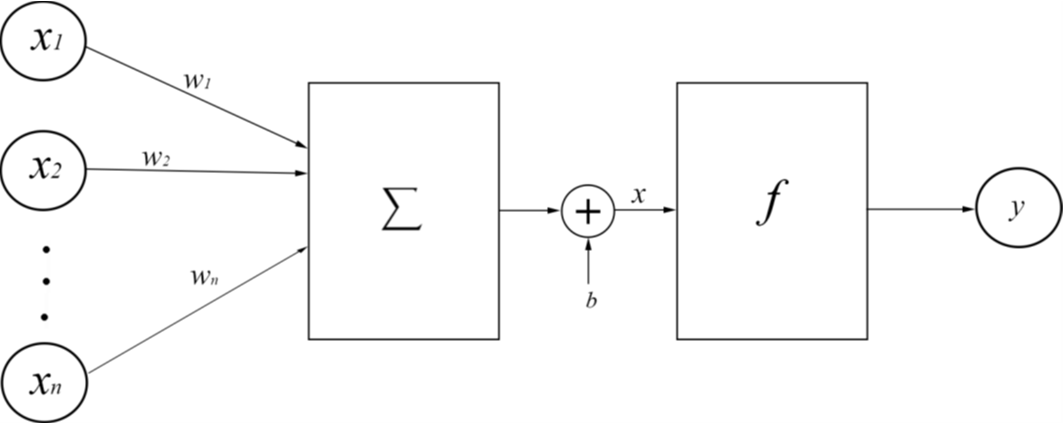
\includegraphics[scale=0.5]{neurone}
        \caption{Modélisation d'un neurone artificiel}
    \end{figure}
    La fonction $f$ , appelée \textbf{fonction d’activation}, est non linéaire. Elle a pour but d’introduire la non-linéarité dans la sortie d’un neurone. Il existe plusieurs fonctions d’activation utilisées dans la pratique:
    \begin{itemize}
        \item \textbf{La fonction sigmoïde}: prend une entrée réelle et la réduit entre 0 et 1. Elle est définie par:
            \begin{equation}
                f(x) = \frac{1}{1 + e^{-x}}
            \end{equation}
        \item \textbf{La fonction tangente hyperbolique}: prend une entrée de valeur réelle et la réduit à une valeur dans $[-1, 1]$. Elle est définie par:
            \begin{equation}
                f(x) = \frac{2}{1 + e^{-2x}} - 1 
            \end{equation}
        \item \textbf{La fonction unité de rectification linéaire (ReLU)}: prend une entrée réelle et retourne cette entrée si elle est positive et 0 sinon:
            \begin{equation}
                f(x) = 
                \begin{cases} 
                    x       & \text{si } x \geq 0 \\
                    0       & \text{si } x < 0
                \end{cases}
            \end{equation}
        \item \textbf{La fonction softmax}: prend un vecteur à valeurs réelles et le réduit à un vecteur de valeurs comprises entre zéro et un qui égal:
            \begin{equation}
                f(x)_{i} = \frac{e^{x_i}}{\sum_{j}e^{x_j}}
            \end{equation}
    \end{itemize}
    En connectant plusieurs neurones, on forme ainsi un réseau de neurones constitué de trois principaux types de couches:
        \begin{itemize}
            \item \textbf{Une couche d'entrée}: Les neurones de cette couche dits d'entrée fournissent des informations du monde extérieur au réseau. Ils transmettent simplement les informations à la prochaine couche.
            \item \textbf{Une ou plusieurs couches cachées}: Les neurones de cette couche dits cachés n'ont aucune connexion directe avec le monde extérieur. Ils effectuent des calculs et transfèrent des informations à la couche suivante.
            \item \textbf{Une couche de sortie}: Les neurones de cette couche dits de sortie sont responsables des calculs et du transfert des informations du réseau vers le monde extérieur.
        \end{itemize}
        \begin{figure}
            \centering
            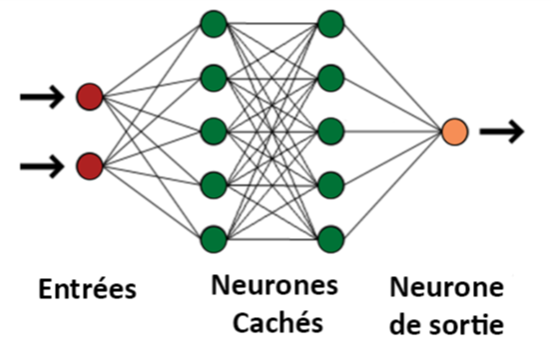
\includegraphics[scale=0.5]{reseauNeurones}
            \caption{Réseau de neurones artificiels}
        \end{figure}
    A partir de l'équation \ref{eq:1}, on peut définir de manière générale un réseau de neurones comme suit.
    Soient:
        \begin{itemize}
            \item $r$ le nombre des neurones sur la couche d’entrée
            \item $s$ le nombre des neurones sur la couche de sortie
            \item $l$ le nombre total des couches du réseau de neurones
            \item $n_k$ le nombre des neurones sur la $k^\text{ème}$ couche avec $0 \leq k \leq l$ tel que $n_0 = r$ et $n_l = s$
            \item les fonctions affines $A_{i}^{k}(x) = \sum_{j = 1}^{n_{k-1}}w_{ij}^{k}x_{j} + b_{j}^{k}$ avec $1 \leq k \leq l$, $1 \leq i \leq n_k$ et $x \in \mathbb{R}^{n_{k-1}}$
            \item $f$ la fonction d’activation du réseau de neurones
            \item le vecteur de sortie $Y = (y_1, ..., y_s)$ défini par la récurrence suivante : 
            \begin{equation}
                \forall x \in \mathbb{R}^{r}, 
                \begin{cases} 
                    a_{0} = x   \\
                    a_{i}^{k} = f(A_{i}^{k}(a^{k-1}))      & \text{avec } 1 \leq k \leq l, 1 \leq i \leq n_k \\
                    y_{i}(x) = A_{i}^{l}(a^{l-1}) & \text{avec } 1 \leq i \leq s
                \end{cases}
            \end{equation}\cite{dahmaneThesis}
        \end{itemize}
    \subsection{Apprentissage d'un réseau de neurones}
    La phase d’apprentissage consiste à ajuster les poids d’un réseau de neurones afin d’obtenir les meilleurs résultats de régression ou de classification dans notre cas. L’objectif de cette optimisation est de minimiser la fonction de coût $\psi$ (\ref{eq:2}) qui calcule l’erreur entre les données de la base d’apprentissage $y$ et les données prédites par le réseau de neurones $\hat{y}$.
    \begin{equation}\label{eq:2}
        \psi(p) = \frac{1}{N}\sum_{i=1}^{N}(y_{i}-\hat{y}_{i})^{2}, \text{ avec } N \text{ le nombre de données d'apprentissage}
    \end{equation}
    L'un des algorithmes d'optimisation proposés dans la litterature est l’algorithme de rétropropagation qui se base sur la \textbf{descente de gradient}. Cet algorithme permet d’approcher son minimum local en cherchant les points auxquels son gradient est nul. Dans le cas des réseaux de neurones, cela signifie que, à chaque itération, la rétropropagation calcule la dérivée de la fonction de coût $\psi$ par rapport à chaque poids et la soustrait de ce dernier selon l’équation:
    \begin{equation}\label{eq:3}
        p_{i+1} = p_{i} - \alpha\bigtriangledown_{p}\psi(p_{i}).
    \end{equation}
    En pratique la base de données d'entraînement est important ($N$ est très grand). A cet effet, on subdivise cette base de données en lots de petite taille appelés \textbf{batchs}. Ainsi l'équation \ref{eq:3} n'est pas appliquée d'un coup sur l'ensemble des données mais sur chaque lot successivement.
    
    Le paramètre $\alpha$ de l’équation \ref{eq:3} est le \textbf{pas de la descente} ou \textbf{learning rate}.C'est l’un des hyperparamètres importants pour l’optimisation des réseaux de neurones profonds en agissant sur sa convergence. En effet, un taux d’apprentissage trop élevé conduit à des mises à jour des poids importantes et la convergence devient instable. Par contre, pour un taux d’apprentissage faible, la convergence est ralentie avec une possibilité de tomber dans des minimas locaux. L’approche populaire utilisée dans l’apprentissage profond pour avoir le taux d’apprentissage optimal est de commencer l’apprentissage avec une valeur élevée afin d’accélérer la descente du gradient et de la réduire par la suite pour améliorer la précision.\cite{dahmaneThesis}
    
    Plusieurs problèmes peuvent être rencontrés lors du processus d'entraînement d'un réseau de neurones. Parmi ceux-ci, nous pouvons citer:
    \begin{itemize}
        \item \textbf{Le surapprentissage}:dans ce cas, le réseau de neurones devient capable de capturer des informations qui ne sont pas utiles pour accomplir sa tâche ou il devient incapable de généraliser les caractéristiques
        des données, ce qui limite sa capacité de reconnaître de nouvelles données. Pour résoudre ce problème, on peut d'une part utiliser la technique \textbf{dropout} qui consiste éliminer certains neurones à chaque itération afin de diminuer le nombre de paramètres du réseau et de mettre à
        jour un nombre réduit de poids. D'autre part, une autre technique consiste à diversifier notre base de données en y ajoutant de nouvelles données.\cite{dahmaneThesis}
        \item \textbf{Le sous-apprentissage}: dans ce cas, le réseau de neurones est incapable de reconnaître même les données d'entraînement. Pour résoudre, on peut entraîner plus longtemps le modèle de réseau de neurones ou encore rendre le réseau de neurones plus complexes en y ajoutant plus de couches cachées.
    \end{itemize}

    Selon le type des données d'entraînement, on distingue des types de réseaux de neurones adaptés à savoir les \acrshort{ann}s, les \acrshort{rnn}s et les \acrshort{cnn}s. Pour un système ANPR qui traite essentiellement les images, les réseaux neurones convolutifs sont les plus adéquats.

    \subsection{Réseaux de neurones convolutifs}
    Aussi appelés \acrshort{cnn} ou ConvNets, les réseaux de neurones convolutifs sont constitués de plusieurs couches empilées. En \citeyear{lenet}, \Citeauthor{lenet}   développent le premier réseau de neurones à convolution appelé LeNet \cite{lenet}. Il servait à reconnaître les caractères comme les codes postaux et les chiffres.
    Pour pouvoir extraire et traiter les caractèristiques des données, les ConvNets se composent des couches suivantes:
        \begin{enumerate}
            \item \textbf{Couche de convolution}:
            Un réseau de neurones convolutif est un réseau de neurones qui utilise une opération mathématique qui s’appelle convolution ou produit de convolution. Il s’agit d’une opération linéaire. Chaque réseau de neurones convolutif contient au moins une couche de convolution. Soient $f$ et $g$ deux fonctions définies sur $\mathbb{R}$, le produit de convolution entre $f$ et $g$ est généralement noté $f*g$  et il est défini par l’équation suivante :
                \begin{equation}
                    (f*g)(x) = \int_{-\infty}^{+\infty} f(t)g(x-t)\,dt 
                \end{equation}
            Dans un réseau de neurones, $f$ est assimilé à l'entrée et $g$ au noyau de convolution. En apprentissage automatique, on utilise en réalité la convolution discrète avec  l'entrée qui est toujours un tableau de données multidimensionnel, et le noyau est toujours un tableau de paramètres multidimensionnel.Dans ce cas, pour une entrée image I et pour un noyau K, la convolution discrète s’écrit:
                \begin{equation}
                    (K*I)(i, j) = \sum_{m}\sum_{n}I(i-m, j-n)K(m, n)
                \end{equation}
            Une couche de convolution est caractérisée par:
                \begin{itemize}
                    \item \textbf{les dimensions des noyaux de convolution}, généralement une convolution à une
                    dimension égale à 2 avec des noyaux carrés.
                    \item \textbf{le nombre des filtres de convolution} $C$, c’est le nombre de cartes d’activations, ou cartes de caractéristiques, en sortie de la couche. Ces cartes sont représentées sous la forme de tenseurs de dimension 3 $(H, W, C)$ avec $H$ la hauteur des cartes, $W$ la largeur et $C$ le nombre de canaux.
                    \item \textbf{le pas de convolution} -ou stride - $s$. C’est le pas de décalage du noyau de convolution à chaque calcul.
                    \item \textbf{le padding} $p$. C’est le paramètre permettant de dépasser la taille de l’image pour
                    appliquer la convolution en ajoutant des pixels autour de l’image.
                \end{itemize}
            \item \textbf{Couche d’échantillonnage (Pooling)}:
            Semblable à la couche de convolution, la couche d’échantillonnage est chargée de réduire la taille spatiale des cartes de caractéristiques, mais elle conserve les informations les plus importantes. Il existe différents types d’échantillonnage dont l’\textbf{échantillonnage maximum -ou Max Pooling-}, l’\textbf{échantillonnage moyen -ou Average Pooling}. Le Max Pooling renvoie la valeur maximale de la partie de l’image couverte par le noyau. Tandis que le Average Pooling prend la moyenne de tous les éléments couverts par le noyau. Si le Average Pooling ne permet juste qu'une réduction dimensionnelle, le Max Pooling par contre est un mecanisme de suppression de bruits. Ceci rend évidemment le Max Pooling plus performant et donc plus utilisé.
            \item \textbf{Couche complètement connectée}:
            La couche complètement connectée est un reseau de neurones multi-couche traditionnel qui utilise une fonction d’activation (par exemple softmax) sur le vecteur de sortie afin d’ajouter la non-linéarité. La sortie des couches de convolution et d’échantillonnage représente des caractéristiques de haut niveau de l’image d’entrée. L’objectif de la couche complètement connectée est d’utiliser ces caractéristiques pour classer l’image d’entrée du réseau en différentes classes en fonction de la base de données d’apprentissage.Les couches entièrement connectées sont généralement suivies d’un dropout. Ce dernier agit sur les poids de ces couches afin de désactiver un certain nombre de neurones pour réduire le nombre de paramètres. Cela permet de contrôler le sur-apprentissage qui peut être causé par un nombre important de paramètres.\cite{dahmaneThesis}
        \end{enumerate}
        \begin{figure}[H]
            \centering
            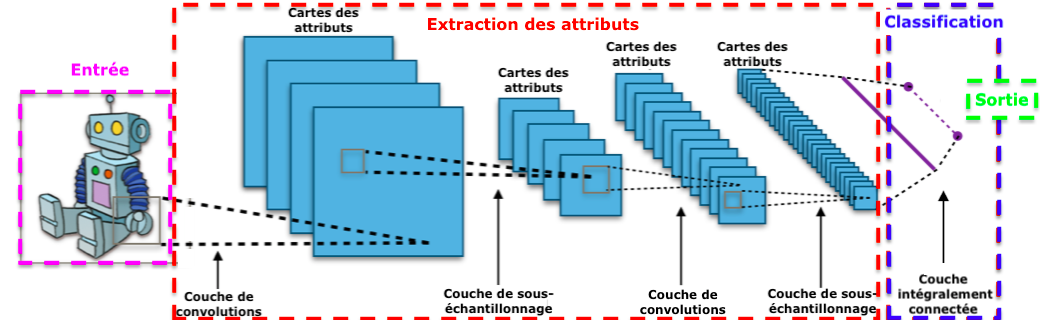
\includegraphics[scale=0.3]{cnn}
            \caption{Architecture d'un réseau de neurones convolutifs}
        \end{figure}
        Parmi les applications où les réseaux de neurones convolutifs sont utilisés avec succès, se trouvent la classification et la détection des objets dans une image. Si construire sa propre architecture CNN de classification des objets est une chose aisée, ce n’est pas le cas pour la détection des objets. En réalité, un réseau de neurones convolutifs dédié à la détection des objets est plus complexe dans son architecture qu’un CNN de classification. C’est la raison pour laquelle plusieurs chercheurs se sont penchés sur la question et ont proposé des algorithmes de création de modèles de détection des objets plus ou moins rapides et précis.
    
    \subsection{Détection des objets}
    Contrairement à la classification, la détection des objets ne se limite pas à reconnaître les objets sur les images. Il faut aller plus loin en les localisant à travers des rectangles appelés \textit{bounding boxes}. Pour y arriver, des spécialistes du domaine de la vision par ordinateur ont mis en place des algorithmes.
        \begin{figure}[H]
            \centering
            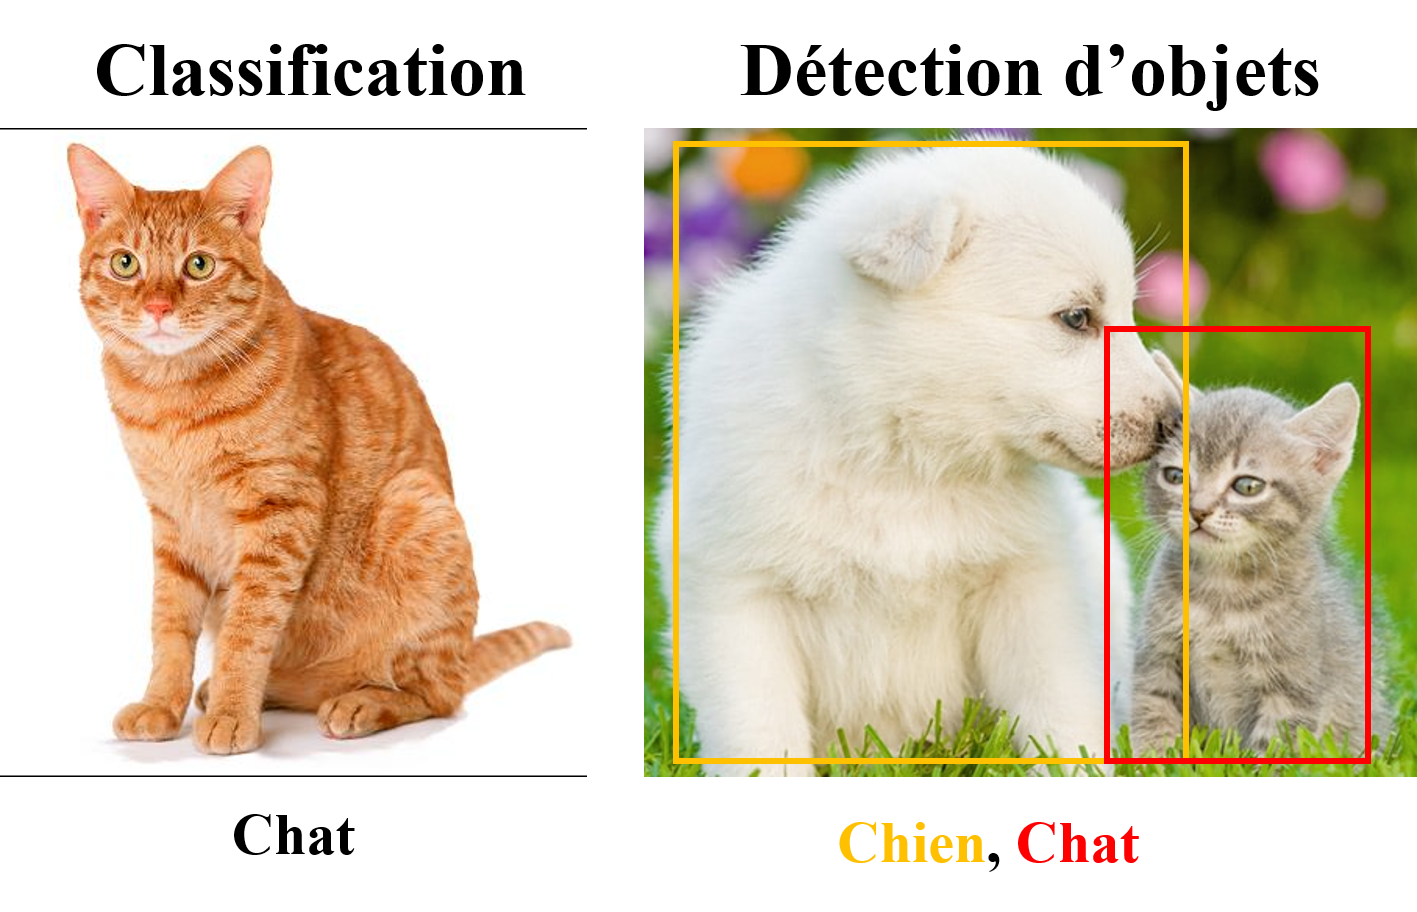
\includegraphics[scale=0.3]{classificationvsobjetDetection}
            \caption{Différence entre classification et détection d'objets}
        \end{figure}
    
    Mais avant de ces algorithmes, commençons par présenter quelques métriques d’évaluation utilisées dans ces algorithmes. 
        \subsubsection{Métriques d'évaluation}
            Les métriques d’évaluation utilisés régulièrement dans les algorithmes de détection d’objets sont:
            \begin{itemize}
                \item \textbf{La précision}: c’est le pourcentage de détections correctes. Il met en évidence l'exactitude des prédictions. Sa formule est:
                \begin{equation}
                    prec = \frac{VP}{VP + FP}
                \end{equation}
            
                \item \textbf{Le rappel}: c’est un indicateur qui mesure la capacité du modèle à prédire l'ensemble des résultats attendus. Ainsi, un modèle peut avoir une très bonne précision mais avoir un mauvais rappel. En effet, un modèle peut-être exact lorsqu'il prédit la présence d'un objet, mais ne pas détecter des objets qui aurait du l'être.
                    \begin{equation}
                        rap = \frac{VP}{VP + FN}
                    \end{equation}
                    \begin{itemize}
                        \item VP: Vrais Positifs, nombre d'objets correctement détectés
                        \item FP: Faux Positifs, nombre d'objets détectés mais non présents en réalité
                        \item FN: Faux Négatifs, nombre d'objets non détectés mais présents en réalité
                    \end{itemize}
            
                \item \textbf{L’intersection sur l’union (\acrshort{iou})}: il permet de comparer la région détectée “prédite” avec la région de la vérité terrain, de manière proportionnelle à la taille de l'objet recherché. Les régions comparées sont les boîtes englobantes : la comparaison des boîtes englobantes permettra de mesurer la qualité de la détection d'objets. Pour cela, on compare l’IoU à un seuil: on considère que l’objet est correctement détecté si et seulement si l’IoU est supérieur au seuil. 
                    \begin{figure}[H]
                        \centering
                        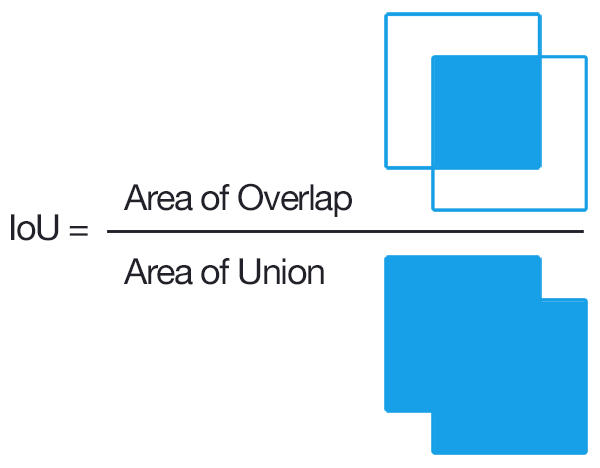
\includegraphics[scale=0.3]{iou_equation}
                        \caption{Equation de l'IoU source: \href{https://www.pyimagesearch.com/2016/11/07/intersection-over-union-iou-for-object-detection/}{pyimagesearch}}
                    \end{figure}
            
                \item \textbf{La précision moyenne (\acrshort{ap})}: A partir de la précision et du rappel, on peut tracer une courbe de précision en fonction du rappel.  L’aire de cette courbe est définie comme la précision moyenne.
            
                \item \textbf{La moyenne de la précision moyenne (\acrshort{map})}:  Si plusieurs valeurs sont choisies pour le seuil de l'IoU, pour chaque classe, l'AP moyenne est calculée sur l'ensemble de ces valeurs seuils et la moyenne des valeurs obtenues donne le mAP. \cite{makina}
                \item \textbf{\acrfull{fps}}: Il répresente le nombre d'images qui peuvent être traitées par seconde. Plus il est grand, plus le modèle de détection est rapide.
            \end{itemize}
    
        \subsubsection{Les algorithmes de détection d'objets}
        Les algorithmes de détection d’objets peuvent être divisés en deux grands groupes. D’une part, nous avons les \textbf{algorithmes de détection à deux étapes}: une étape de détection de régions possibles d’objets possibles en utilisant, une étape pour classer l’objet éventuel dans chaque région. D’autre part, nous retrouvons les \textbf{algorithmes de détection à une étape} qui fait la détection des objets par un seul passage dans un réseau de neurones. Dans le premier groupe, on a les algorithmes comme \textbf{\acrshort{rcnn}, Fast R-CNN, Faster R-CNN}. Dans le second groupe, on y trouve \textbf{\acrshort{yolo}, \acrshort{ssd}}. Décrivons brièvement certains de ces algorithmes.
        \begin{itemize}
            \item \acrfull{rcnn}: Il a été proposé par \citeauthor{rcnn}. A partir d’un algorithme de recherche selective, on extrait sur l’image à traiter 2000 régions appélées régions de propositions. Chacune de ces régions est par la suite introduite dans un CNN pour en extraire les caractéristiques. Ces caractéristiques sont envoyées à un SVM qui classe la présence d’un objet sur la région candidate. En outre, l’algorithme prédit 4 valeurs dites de décalage pour la précision du cadre de délimitation.
                \begin{figure}[H]
                    \centering
                    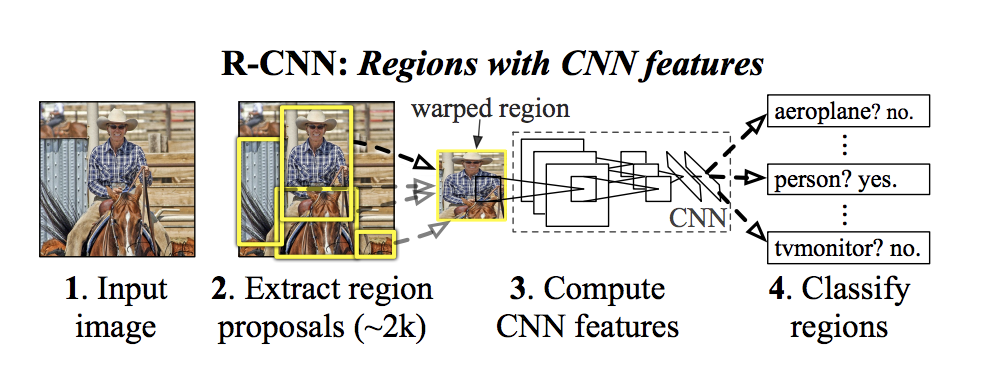
\includegraphics[scale=0.4]{rcnn}
                    \caption{R-CNN}
                \end{figure}
            \item \textbf{Fast R-CNN}: Le même auteur de R-CNN a résolu certains des inconvénients de celui-ci en créant un algorithme de détection d'objets plus rapide appelé Fast R-CNN. L'approche est similaire à l'algorithme R-CNN. Mais, au lieu de fournir les propositions de région au CNN, nous transmettons l'image d'entrée au CNN pour générer une carte de caractéristiques convolutives. À partir de la carte des caractéristiques convolutives, nous identifions la région des propositions et les déformons en carrés et en utilisant une couche de regroupement de RoI, nous les remodelons en une taille fixe afin qu'elle puisse être introduite dans une couche entièrement connectée. À partir du vecteur de caractéristiques RoI, nous utilisons une couche softmax pour prédire la classe de la région proposée ainsi que les valeurs de décalage pour la boîte englobante.
                \begin{figure}[H]
                    \centering
                    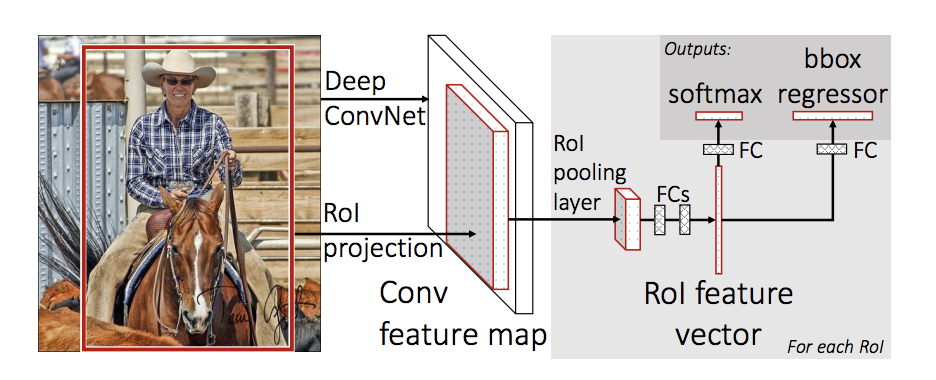
\includegraphics[scale=0.4]{fastrcnn}
                    \caption{Fast R-CNN}
                \end{figure}
            \item \textbf{Faster-RCNN}:Les deux algorithmes ci-dessus (R-CNN et Fast R-CNN) utilisent une recherche sélective pour trouver les propositions de région. La recherche sélective est un processus lent et fastidieux qui affecte les performances du réseau. A la place de cette recherche, \citeauthor{rcnnfaster} ont proposé un réseau de neurones convolutifs appelé \acrfull{rpn} qui prédit les propositions de région. Le reste des étapes est le même que celui d'un Fast-RCNN décrit plus haut.
                \begin{figure}[H]
                    \centering
                    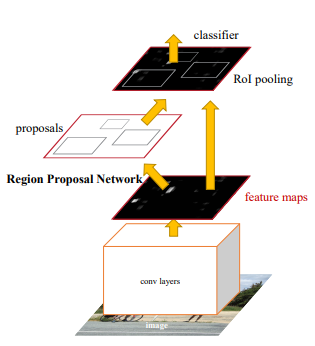
\includegraphics[scale=0.6]{fasterrcnn}
                    \caption{Faster R-CNN}
                \end{figure}
            \item \acrfull{ssd}: En fin novembre 2016, \citeauthor{ssd}publient un article portant sur un nouvel algorithme de détection à une seule étape qu’ils choisissent d’appeler \acrshort{ssd}. Cet algorithme permet de créer des modèles qui atteignent des précisions record par rapport à Faster R-CNN: 74.3\% mAP à 59 FPS \cite{ssd} sur les jeux de données populaires comme Pascal VOC. L’architecture SSD est composée de deux parties: un \textbf{modèle de base} et une \textbf{tête SSD}. Le modèle de base est généralement un réseau de classification d'images pré-entraîné pour extraire les caractéristiques. La tête SSD est constituée d’une ou plusieurs couches convolutives ajoutées à la première partie et les sorties sont interprétées comme les cadres de délimitation et les classes d'objets. Dans la figure ci-dessous le modèle de base est représenté par les boîtes blanches tandis que la tête SSD est représentée par les boîtes bleues.
                \begin{figure}
                    \centering
                    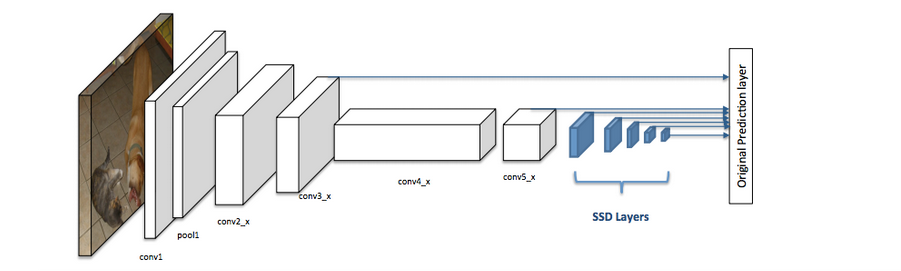
\includegraphics[scale=0.4]{ssd}
                    \caption{Architecture du SSD}
                \end{figure}

            \item \acrfull{yolo}: En \citeyear{redmon2016look}, \citeauthor{redmon2016look} proposent une nouvelle approche qui permet de détecter les objets en prenant l’image en entier et en une seule instance. Ce qui justifie le nom donné à l’algorithme You Only Look Once qui signifie littéralement On ne regarde qu’une seule fois. Contrairement à Faster R-CNN, YOLO utilise un seul réseau convolutif pour prédire en même temps les boîtes englobantes (bounding boxes) et les probabilités de classe pour ces boîtes.
            De manière concrète et simple, on peut résumer le fonctionnement de YOLO comme suit:
                \begin{enumerate}
                    \item YOLO prend en entrée une image
                    \item Il divise l’image en une grille SXS
                    \item La classification et la localisation des images sont effectuées sur chaque grille. Par après, YOLO prédit les cadres de délimitation et leurs probabilités de classe correspondantes pour les objets. 
                \end{enumerate}
                \begin{figure}[H]
                    \centering
                    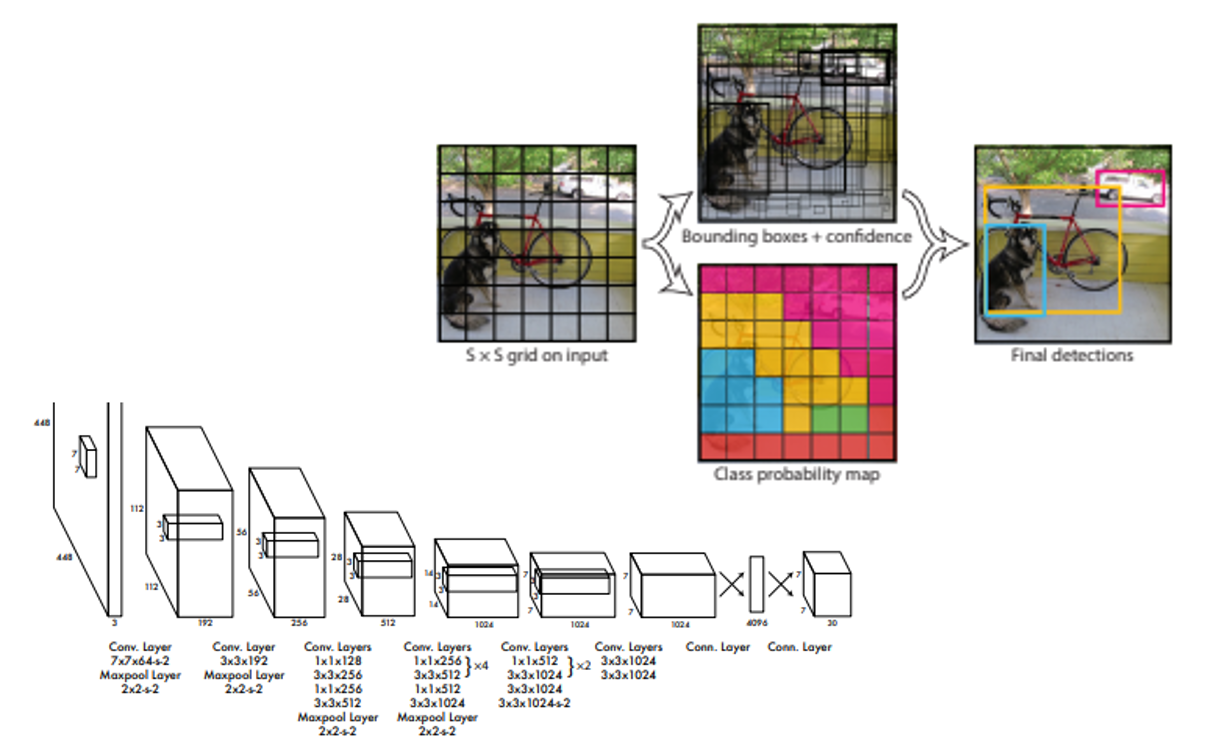
\includegraphics[scale=0.4]{yolov1}
                    \caption{Architecture de la première de version de YOLO}
                \end{figure}
            L’un des problèmes qui peut arriver avec YOLO comme la plupart des algorithmes de détection des objets est qu’un même objet est détecté plus d’une fois. Pour résoudre ce problème, on fait appel à l’algorithme NMS (Non Max Suppression) qui supprime les doublons de détections du même objet. L’algorithme est décrit
                
            \begin{figure}[H]
                \centering
                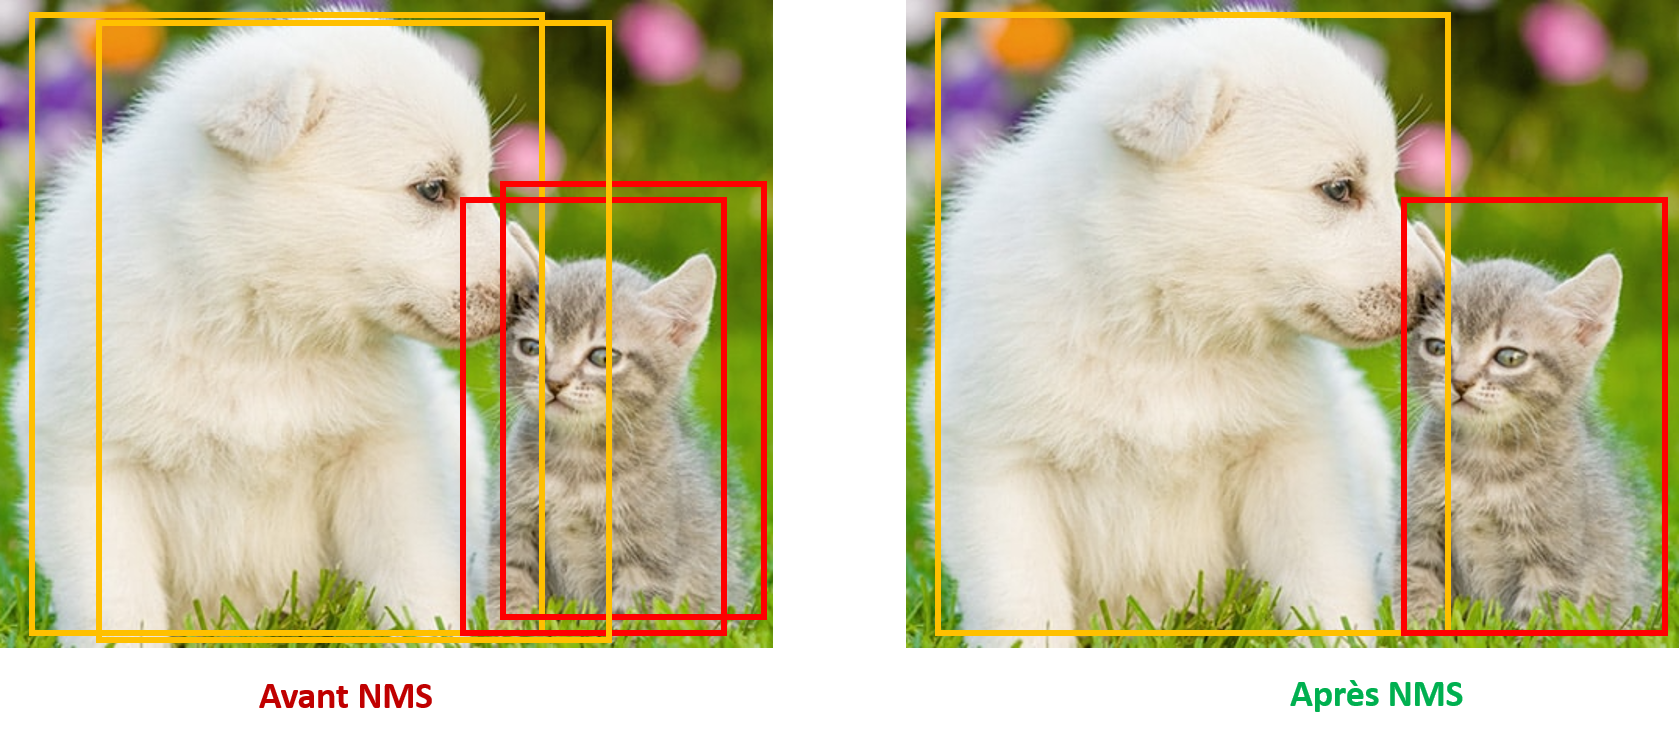
\includegraphics[scale=0.4]{nms}
                \caption{NMS}
            \end{figure}

            \begin{algorithm}[H]
                \caption{Non Max Suppression}
                \begin{algorithmic}[1]
                \Function{nms}{$\mathcal{B}, \mathcal{S}, \mathcal{N}_s$} \Comment{$\mathcal{B}$:cadres initiaux, $\mathcal{S}$:scores initiaux, $\mathcal{N}_s$: seuil de NMS}
                    \State $\mathcal{B}_{nms} \leftarrow \emptyset$
                    \While{$\mathcal{B} \not= \emptyset$}  
                        \State $m \leftarrow findMax(\mathcal{S})$  \Comment{Recherche de l'indice du cadre de plus haut score}
                        \State $b_{max} \leftarrow \mathcal{B}[m]$
                        \For{$b_i \in \mathcal{B}$}
                            \If{$iou(b_{max}, b_i) \geq \mathcal{N}_s$}\Comment{On élimine tout cadre très proche du cadre actuel}
                                \State $\mathcal{B} \leftarrow \mathcal{B} - b_i$
                                \State $\mathcal{S} \leftarrow \mathcal{S} - s_i$
                            \EndIf
                        \EndFor
                        \State $\mathcal{B}_{nms} \leftarrow \mathcal{B}_{nms} \bigcup b_{max}$
                    \EndWhile 
                    \State \Return $\mathcal{B}_{nms}, \mathcal{S}$
                \EndFunction
                \end{algorithmic}
            \end{algorithm}
            Après la première version de YOLO, d’autres nouvelles versions ont été développées pour augmenter les performances des modèles de détection d’objets. Ci-dessous se trouve le tableau comparatif des différentes versions de YOLO fait dans le cadre d’une étude réalisée par des chercheurs tunisiens sur la détection des plaques de véhicules.
            \begin{table}[H]
                \centering
                \begin{tabular}{|l|l|l|l|l|l|l|}
                    \hline
                    \rowcolor{Gray}
                    \textbf{YOLO} & \textbf{v2} & \textbf{v3} & \textbf{v3-tiny} & \textbf{v3-SPP} & \textbf{v4} & \textbf{v4-tiny} \\ \hline
                    Anchors  & 5 & 9 & 6 & 9 & 9 & 6 \\ \hline
                    Backbone & VGG-16 & Darknet-53 & Darknet-19 & Darknet-53 & CSPDarknet-53 & CSPNet-15 \\ \hline
                    FPN & Absent & Présent & Présent & Présent & Présent & Présent \\ \hline
                    SPP & Absent & Absent & Absent & Présent & Présent & Présent \\ \hline
                    PAN & Absent & Absent & Absent & Absent & Présent & Présent \\ \hline
                    mAP@0.5(\%) & 44.0 & 55.3 & 33.1 & 60.6 & 62.8 & 40.2 \\ \hline
                    Vitesse (FPS) & 40 & 66 & 345 & 38 & 55 & 330 \\ \hline
                    Taille (MB) & 275 & 236 & 33.7 & 240 & 245 & 23.1 \\ \hline
                \end{tabular}
                \caption{Comparaison entre les différentes versions de YOLO}
                \label{table:yolo}
            \end{table}
            
        \end{itemize}
